\section{Descriptive figures}\label{sec:data:figures}
\texttt{python/paper/figuresDataNote.py} draws the three figures from \texttt{data/oecd26\_theta.csv} alone.

\begin{figure}[htbp]
\centering
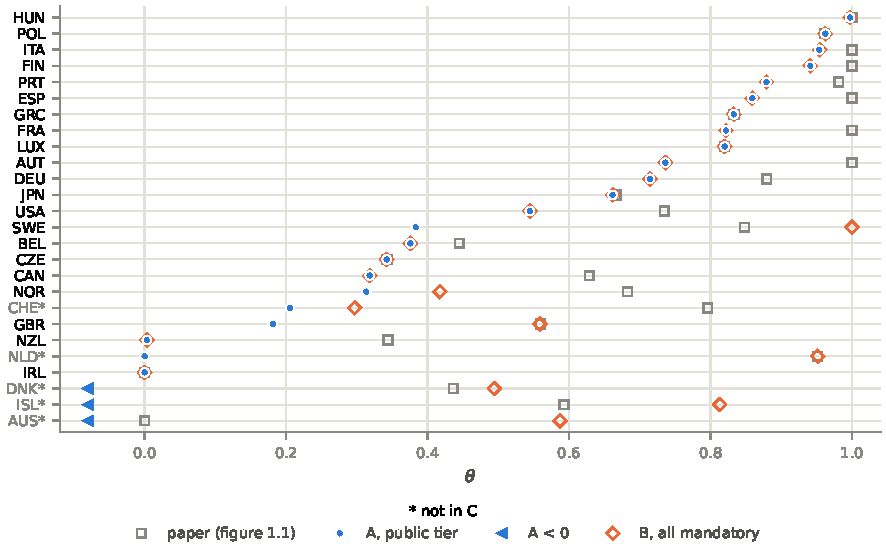
\includegraphics[width=\linewidth]{figs/dataThetaVariants.pdf}
\caption{$\theta$ by country under the paper's index, A and B, sorted by A. A star marks the five countries C drops; a triangle at the left edge marks a negative A slope.}\label{fig:data:thetaVariants}
\end{figure}

\smalltitle{$\theta$ by variant} (\cref{fig:data:thetaVariants}). The paper's index puts six countries at $\theta = 1$ (AUT, ESP, FIN, FRA, HUN, ITA) and two at 0 (AUS, IRL). Under A only HUN stays at the top corner (0.997); ITA (0.954) and FIN (0.941) come close, and AUT falls to 0.736. The bottom corner gains NLD and NZL (0.003, the flat NZ Super read at 0.6 AW), and AUS, DNK and ISL fall below it, since their public pensions are tested against the funded ones. B mostly restores the paper's index where private tiers are large (NLD 0.952, GBR 0.559) and exceeds it in SWE (1, clipped) and ISL (0.813 against 0.593).

\begin{figure}[htbp]
\centering
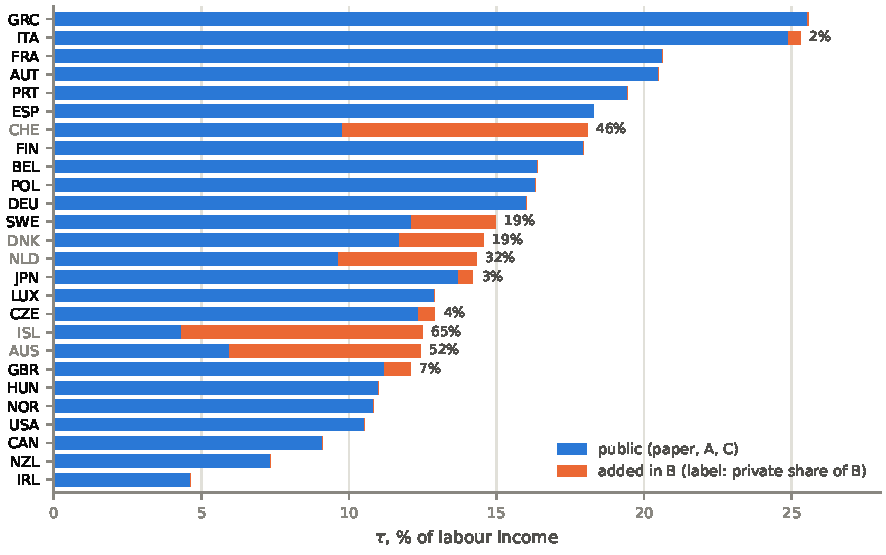
\includegraphics[width=\linewidth]{figs/dataTauVariants.pdf}
\caption{$\tau$ by country: the public system (paper, A, C) and the private spending B adds, labelled with B's private share $\pi$ (\cref{eq:data:SB}). Countries C drops in grey.}\label{fig:data:tauVariants}
\end{figure}

\smalltitle{$\tau$ by variant} (\cref{fig:data:tauVariants}). The public $\tau$ runs from 4.3\% of labour income in ISL to 25.5\% in GRC. B nearly triples it in ISL (to 12.5\%, $\pi = 0.65$), doubles it in AUS (5.9 to 12.4\%, $\pi = 0.52$) and nearly doubles it in CHE (9.8 to 18.1\%, $\pi = 0.46$); it raises it by about half in NLD (9.7 to 14.3\%) and by a quarter in DNK and SWE ($\pi = 0.19$ in both). Elsewhere the private share is below 0.08. The five countries above C's threshold of 0.25 are the five C drops.

\begin{figure}[htbp]
\centering
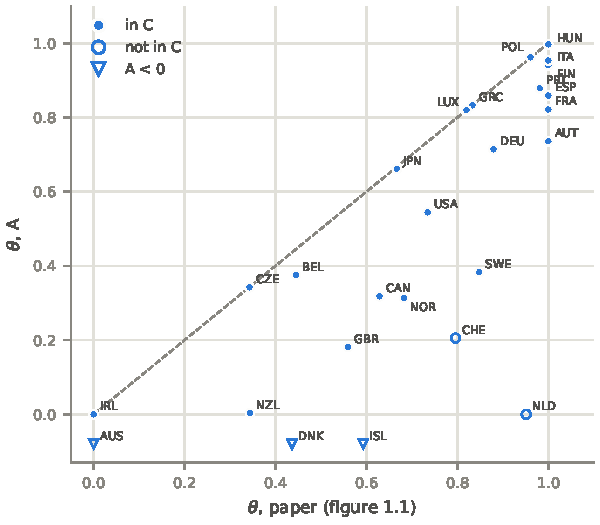
\includegraphics[width=0.62\linewidth]{figs/dataThetaPaperA.pdf}
\caption{$\theta$ under A against the paper's index, with the $45^\circ$ line. Hollow: not in C; triangles: negative A slope, drawn at the bottom edge.}\label{fig:data:thetaPaperA}
\end{figure}

\smalltitle{The paper's $\theta$ against A} (\cref{fig:data:thetaPaperA}). Every country lies on or below the $45^\circ$ line (POL 0.962 against 0.961 is rounding). The two measures agree where the public tier is the mandatory system and its formula is close to linear (CZE, GRC, HUN, JPN, LUX, POL). A lies below where a flat tier or a minimum sits under the earnings-related one: the paper's six countries at $\theta = 1$ spread over 0.736 (AUT) to 0.997 (HUN), and the U.S.\ falls from 0.735 to 0.544, because the point at 2 AW lies above the PIA's upper bend point (A2pt gives 0.728). The largest gaps are the private-tier countries: NLD (0.951 to 0), CHE (0.796 to 0.205) and SWE (0.848 to 0.383). On the 23 countries with a value, A averages 0.559 against the paper's 0.760, and the two correlate at 0.72.
